\documentclass[utf8, russian]{beamer}

\usepackage[utf8]{inputenc}
\usepackage[russian]{babel}
\usepackage{hyperref}
\usepackage{graphicx}
\usepackage{listings}
\usepackage{ucs}

\lstset{
    extendedchars=\true,
    inputencoding=utf8x
}

\usetheme{Warsaw}
\usecolortheme{lily}
\useoutertheme[subsection=false]{smoothbars}
\useinnertheme{circles}
\setbeamertemplate{footline}[page number]{}
\setbeamertemplate{navigation symbols}{}

\renewcommand{\figurename}{} 

\title{Архитектура ЭВМ}
\subtitle{Лекция 5. Стек и подпрограммы}
\author{к.ф.-м.н. Филонов Павел Владимирович \\ filonovpv@gmail.com}
\date{22 сентября 2013 г.}


\institute[МГТУ ГА] 
{
    Московский Государственный Технический Университет \\
    Гражданской Авиации
}
\begin{document}
    \frame{\titlepage}
    \begin{frame}{Стек}

        {\bf Стек } ({\it англ.} Stack) --- структура данных, организованная по принципу LIFO (Last In --- First Out, последнием пришёл --- первым вышел)
    \begin{columns}
        \column{0.5\linewidth}
            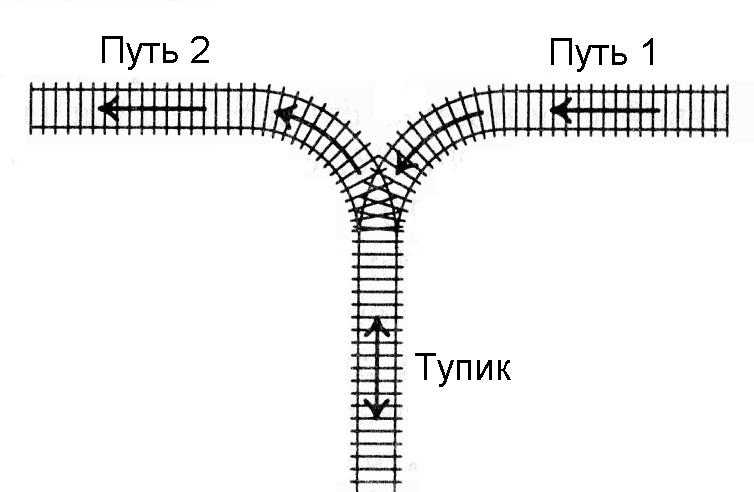
\includegraphics[width=\linewidth]{fig/stack_rails.jpg}
        \column{0.5\linewidth}
            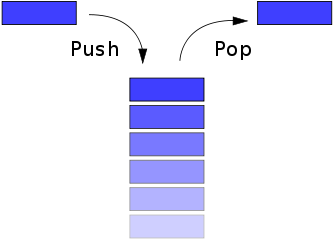
\includegraphics[width=\linewidth]{fig/stack.png}
    \end{columns}
    {\bf Push} --- положить элемент на вершину стека

    {\bf Pop} --- снять элемент с вершины стека
    \end{frame}
    \begin{frame}{Организация стека в архитектуре x86}
        \begin{columns}
        \column{0.5\linewidth}
        \begin{itemize}
            \item Секция стека располагается в старших адресах памяти. 
            \item Адрес вершины стека хранится в регисре ESP.
            \item Вершина стека растёт в сторону уменьшения адресов. 
        \end{itemize}
        \column{0.5\linewidth}
        
    \end{frame}
\end{document}